\PassOptionsToPackage{unicode=true}{hyperref} % options for packages loaded elsewhere
\PassOptionsToPackage{hyphens}{url}
%
\documentclass[a4paper]{article}
\usepackage{lmodern}
\usepackage{amssymb,amsmath}
\usepackage{ifxetex,ifluatex}
\usepackage{fixltx2e} % provides \textsubscript
\ifnum 0\ifxetex 1\fi\ifluatex 1\fi=0 % if pdftex
  \usepackage[T1]{fontenc}
  \usepackage[utf8]{inputenc}
  \usepackage{textcomp} % provides euro and other symbols
\else % if luatex or xelatex
  \usepackage{unicode-math}
  \defaultfontfeatures{Ligatures=TeX,Scale=MatchLowercase}
\fi
% use upquote if available, for straight quotes in verbatim environments
\IfFileExists{upquote.sty}{\usepackage{upquote}}{}
% use microtype if available
\IfFileExists{microtype.sty}{%
\usepackage[]{microtype}
\UseMicrotypeSet[protrusion]{basicmath} % disable protrusion for tt fonts
}{}
\IfFileExists{parskip.sty}{%
\usepackage{parskip}
}{% else
\setlength{\parindent}{0pt}
\setlength{\parskip}{6pt plus 2pt minus 1pt}
}
\usepackage{hyperref}
\hypersetup{
            pdftitle={Linear Regression Analysis of Electricity Consumption},
            pdfauthor={Edward J. Xu (edxu96@outlook.com)},
            pdfborder={0 0 0},
            breaklinks=true}
\urlstyle{same}  % don't use monospace font for urls
\usepackage{color}
\usepackage{fancyvrb}
\newcommand{\VerbBar}{|}
\newcommand{\VERB}{\Verb[commandchars=\\\{\}]}
\DefineVerbatimEnvironment{Highlighting}{Verbatim}{commandchars=\\\{\}}
% Add ',fontsize=\small' for more characters per line
\usepackage{framed}
\definecolor{shadecolor}{RGB}{248,248,248}
\newenvironment{Shaded}{\begin{snugshade}}{\end{snugshade}}
\newcommand{\AlertTok}[1]{\textcolor[rgb]{0.94,0.16,0.16}{#1}}
\newcommand{\AnnotationTok}[1]{\textcolor[rgb]{0.56,0.35,0.01}{\textbf{\textit{#1}}}}
\newcommand{\AttributeTok}[1]{\textcolor[rgb]{0.77,0.63,0.00}{#1}}
\newcommand{\BaseNTok}[1]{\textcolor[rgb]{0.00,0.00,0.81}{#1}}
\newcommand{\BuiltInTok}[1]{#1}
\newcommand{\CharTok}[1]{\textcolor[rgb]{0.31,0.60,0.02}{#1}}
\newcommand{\CommentTok}[1]{\textcolor[rgb]{0.56,0.35,0.01}{\textit{#1}}}
\newcommand{\CommentVarTok}[1]{\textcolor[rgb]{0.56,0.35,0.01}{\textbf{\textit{#1}}}}
\newcommand{\ConstantTok}[1]{\textcolor[rgb]{0.00,0.00,0.00}{#1}}
\newcommand{\ControlFlowTok}[1]{\textcolor[rgb]{0.13,0.29,0.53}{\textbf{#1}}}
\newcommand{\DataTypeTok}[1]{\textcolor[rgb]{0.13,0.29,0.53}{#1}}
\newcommand{\DecValTok}[1]{\textcolor[rgb]{0.00,0.00,0.81}{#1}}
\newcommand{\DocumentationTok}[1]{\textcolor[rgb]{0.56,0.35,0.01}{\textbf{\textit{#1}}}}
\newcommand{\ErrorTok}[1]{\textcolor[rgb]{0.64,0.00,0.00}{\textbf{#1}}}
\newcommand{\ExtensionTok}[1]{#1}
\newcommand{\FloatTok}[1]{\textcolor[rgb]{0.00,0.00,0.81}{#1}}
\newcommand{\FunctionTok}[1]{\textcolor[rgb]{0.00,0.00,0.00}{#1}}
\newcommand{\ImportTok}[1]{#1}
\newcommand{\InformationTok}[1]{\textcolor[rgb]{0.56,0.35,0.01}{\textbf{\textit{#1}}}}
\newcommand{\KeywordTok}[1]{\textcolor[rgb]{0.13,0.29,0.53}{\textbf{#1}}}
\newcommand{\NormalTok}[1]{#1}
\newcommand{\OperatorTok}[1]{\textcolor[rgb]{0.81,0.36,0.00}{\textbf{#1}}}
\newcommand{\OtherTok}[1]{\textcolor[rgb]{0.56,0.35,0.01}{#1}}
\newcommand{\PreprocessorTok}[1]{\textcolor[rgb]{0.56,0.35,0.01}{\textit{#1}}}
\newcommand{\RegionMarkerTok}[1]{#1}
\newcommand{\SpecialCharTok}[1]{\textcolor[rgb]{0.00,0.00,0.00}{#1}}
\newcommand{\SpecialStringTok}[1]{\textcolor[rgb]{0.31,0.60,0.02}{#1}}
\newcommand{\StringTok}[1]{\textcolor[rgb]{0.31,0.60,0.02}{#1}}
\newcommand{\VariableTok}[1]{\textcolor[rgb]{0.00,0.00,0.00}{#1}}
\newcommand{\VerbatimStringTok}[1]{\textcolor[rgb]{0.31,0.60,0.02}{#1}}
\newcommand{\WarningTok}[1]{\textcolor[rgb]{0.56,0.35,0.01}{\textbf{\textit{#1}}}}
\usepackage{longtable,booktabs}
% Fix footnotes in tables (requires footnote package)
\IfFileExists{footnote.sty}{\usepackage{footnote}\makesavenoteenv{longtable}}{}
\usepackage{graphicx,grffile}
\makeatletter
\def\maxwidth{\ifdim\Gin@nat@width>\linewidth\linewidth\else\Gin@nat@width\fi}
\def\maxheight{\ifdim\Gin@nat@height>\textheight\textheight\else\Gin@nat@height\fi}
\makeatother
% Scale images if necessary, so that they will not overflow the page
% margins by default, and it is still possible to overwrite the defaults
% using explicit options in \includegraphics[width, height, ...]{}
\setkeys{Gin}{width=\maxwidth,height=\maxheight,keepaspectratio}
\setlength{\emergencystretch}{3em}  % prevent overfull lines
\providecommand{\tightlist}{%
  \setlength{\itemsep}{0pt}\setlength{\parskip}{0pt}}
\setcounter{secnumdepth}{0}
% Redefines (sub)paragraphs to behave more like sections
\ifx\paragraph\undefined\else
\let\oldparagraph\paragraph
\renewcommand{\paragraph}[1]{\oldparagraph{#1}\mbox{}}
\fi
\ifx\subparagraph\undefined\else
\let\oldsubparagraph\subparagraph
\renewcommand{\subparagraph}[1]{\oldsubparagraph{#1}\mbox{}}
\fi

% set default figure placement to htbp
\makeatletter
\def\fps@figure{htbp}
\makeatother


\title{Linear Regression Analysis of Electricity Consumption}
\author{Edward J. Xu
(\href{mailto:edxu96@outlook.com}{\nolinkurl{edxu96@outlook.com}})}
\date{2020-04-05}

\begin{document}
\maketitle

\hypertarget{latest-updates}{%
\subsection{Latest Updates}\label{latest-updates}}

\begin{itemize}
\tightlist
\item
  The value 1 of \texttt{x5} will indicate a female respondent, while
  male respondents are represented using 0 instead 2. This modification
  will make it easier to intepret the intercepts in models containing
  \texttt{x5}.
\item
  Correct the degree of freedom in White's test for
  \texttt{mods{[}{[}5{]}{]}}.
\item
  Add hand-calculation RESET test and JB test.
\item
  Update section 8 causality.
\item
  Present the final model \texttt{mods{[}{[}7{]}{]}}.
\item
  Discuss why we choose the final model in detail.
\item
  Interpret the final model using economics.
\item
  Correct some small written mistakes.
\item
  Add more comments on the data set and final results.
\item
  Add hand-written calculation for likelihood tests.
\item
  Add subsection 10-3 orthogonalization of multiple regressors.
\item
  Talk about model selection in more detail.
\end{itemize}

\hypertarget{introduction}{%
\subsection{Introduction}\label{introduction}}

Following packages and functions are used in this project.

\begin{Shaded}
\begin{Highlighting}[]
\CommentTok{## basic packages}
\KeywordTok{library}\NormalTok{(knitr)}
\KeywordTok{library}\NormalTok{(kableExtra)}
\KeywordTok{library}\NormalTok{(tidyverse)}
\KeywordTok{library}\NormalTok{(conflicted)}
\KeywordTok{library}\NormalTok{(magrittr)}
\KeywordTok{library}\NormalTok{(broom)}
\CommentTok{# library(car)}
\CommentTok{## paticular packages for this project}
\KeywordTok{library}\NormalTok{(lmtest)}
\KeywordTok{library}\NormalTok{(corrr)}
\KeywordTok{library}\NormalTok{(tseries)}
\KeywordTok{library}\NormalTok{(corrplot)}
\KeywordTok{source}\NormalTok{(}\StringTok{"./funcs.R"}\NormalTok{)}
\end{Highlighting}
\end{Shaded}

The data set is defined as follows based on file \texttt{recs.csv}:

\begin{Shaded}
\begin{Highlighting}[]
\KeywordTok{set.seed}\NormalTok{(}\DecValTok{6}\NormalTok{)}
\NormalTok{dat <-}\StringTok{ }
\StringTok{  }\KeywordTok{read_csv}\NormalTok{(}\StringTok{"./data/recs.csv"}\NormalTok{) }\OperatorTok
\StringTok{  }\NormalTok{dplyr}\OperatorTok{::}\KeywordTok{slice}\NormalTok{(}\KeywordTok{sample}\NormalTok{(}\KeywordTok{nrow}\NormalTok{(.), }\DecValTok{300}\NormalTok{)) }\OperatorTok
\StringTok{  }\KeywordTok{mutate}\NormalTok{(}\DataTypeTok{y =} \KeywordTok{log}\NormalTok{(KWH }\OperatorTok{/}\StringTok{ }\NormalTok{NHSLDMEM)) }\OperatorTok
\StringTok{  }\KeywordTok{mutate}\NormalTok{(}\DataTypeTok{x8 =}\NormalTok{ TOTROOMS }\OperatorTok{+}\StringTok{ }\NormalTok{NCOMBATH }\OperatorTok{+}\StringTok{ }\NormalTok{NHAFBATH) }\OperatorTok
\StringTok{  }\NormalTok{dplyr}\OperatorTok{::}\KeywordTok{select}\NormalTok{(y, }\DataTypeTok{x2 =}\NormalTok{ NHSLDMEM, }\DataTypeTok{x3 =}\NormalTok{ EDUCATION, }\DataTypeTok{x4 =}\NormalTok{ MONEYPY, }\DataTypeTok{x5 =}\NormalTok{ HHSEX, }
    \DataTypeTok{x6 =}\NormalTok{ HHAGE, }\DataTypeTok{x7 =}\NormalTok{ ATHOME, x8) }\OperatorTok
\StringTok{  }\KeywordTok{mutate_at}\NormalTok{(}\KeywordTok{seq}\NormalTok{(}\DecValTok{2}\NormalTok{, }\DecValTok{8}\NormalTok{), as.integer) }\OperatorTok\StringTok{  }\CommentTok{# make continuous variables discrete}
\StringTok{  }\KeywordTok{mutate}\NormalTok{(}\DataTypeTok{x5 =} \OperatorTok{-}\StringTok{ }\NormalTok{x5 }\OperatorTok{+}\StringTok{ }\DecValTok{2}\NormalTok{) }
\end{Highlighting}
\end{Shaded}

Different variables are summarized in the following table. \texttt{y},
the logarithm of averaged electricity consumption, is the variable that
we are interested in. Specifically, The electricity consumption refers
to the electricity usage of the house/studio where the respondent lives
in 2015, measured in kilowatthours. The quantity is average by the
number of household members in the house/studio. That way, it roughly
represent the level of electricity consumption of the respondent. Other
variables are discussion in the following table.

\begin{longtable}[]{@{}lll@{}}
\toprule
Sym & Abbr & Definition\tabularnewline
\midrule
\endhead
z & KWH & electricity consumption\tabularnewline
y & LKWH.pers & logarithm of KWH/NHSLDMEM\tabularnewline
x2 & NHSLDMEM & number of household members\tabularnewline
x3 & EDUCATION & highest education completed\tabularnewline
x4 & MONEYPY & annual gross household income last year\tabularnewline
x5 & HHSEX & gender\tabularnewline
x6 & HHAGE & age\tabularnewline
x7 & ATHOME & number of weekdays someone is at home\tabularnewline
x8 & TOTROOMS + & number of rooms (including bathrooms)\tabularnewline
\bottomrule
\end{longtable}

Note that \texttt{x8} is a variable indicating the number of rooms of
the house/studio of the respondent. It equals the summation of
\texttt{TOTROOMS}, \texttt{NCOMBATH} and \texttt{NHAFBATH} in the
original data set. \texttt{x8} is not included in the initial analysis
(sections 1 to 7).

\texttt{x3}, the education level of the respondent, is considered as a
continuous variable in this project for simplicity. The detailed
definition of different levels is shown in the following table.

\begin{longtable}[]{@{}ll@{}}
\toprule
Level & Definition\tabularnewline
\midrule
\endhead
1 & Less than high school diploma or GED\tabularnewline
2 & High school diploma or GED\tabularnewline
3 & Some college or Associate's degree\tabularnewline
4 & Bachelor's degree (for example: BA, BS)\tabularnewline
5 & Master's, Professional, or Doctorate degree\tabularnewline
\bottomrule
\end{longtable}

The first 5 rows of the data set used can be visualized:

\begin{table}[H]
\centering
\begin{tabular}{llllllll}
\toprule
y & x2 & x3 & x4 & x5 & x6 & x7 & x8\\
\midrule
7.5 & 5 & 3 & 8 & 1 & 39 & 5 & 15\\
8.2 & 1 & 2 & 2 & 0 & 85 & 5 & 14\\
8.7 & 3 & 1 & 1 & 0 & 71 & 5 & 8\\
7.8 & 4 & 3 & 5 & 1 & 39 & 5 & 8\\
9.8 & 1 & 3 & 3 & 0 & 57 & 0 & 10\\
\bottomrule
\end{tabular}
\end{table}

In this project, we want to develop a model associating the continuous
variable, average electricity consumption, with other variables. We will
start by visualizing correlations between variables. In particular, the
two variables \texttt{x2} and \texttt{x6}, which highly correlate with
\texttt{y} will be explored. The model regressing \texttt{y} on
\texttt{x2} will be discussed in section 2. Four assumptions will be
made, three of which will be tested in section 3-5 by Jarque-Bera test
(normality), White's test (homoskedasticity) and RESET test (functional
form) respectively. According the test results and discussion in section
6, data point \texttt{36} is excluded. Then, in section 7, more
regressors are introduced and three new models are established. The
detail regarding how regressors interact with each other, namely
causality, is discussed in section 8. Based on the understanding of the
underlying mechanism, a nonlinear term and \texttt{x8} are included as
new regressors. Two new models are estimated, based on the only model
passing all tests in section 7. Finally, the model called
\texttt{mods{[}{[}7{]}{]}} is chosen as the final for presentation and
it is interpreted in section 10.

\hypertarget{data-visualization}{%
\subsection{1. Data Visualization}\label{data-visualization}}

It can be seen that \texttt{y} is highly correlated to \texttt{x2} and
\texttt{x6} according to the following table.

\begin{table}[H]
\centering
\begin{tabular}{lll}
\toprule
x & y & r\\
\midrule
x2 & y & -0.511\\
x3 & y & 0.034\\
x4 & y & 0.041\\
x5 & y & -0.043\\
x6 & y & 0.353\\
x7 & y & 0.040\\
x8 & y & 0.213\\
\bottomrule
\end{tabular}
\end{table}

It can be seen from the following covariance matrix that \texttt{y} is
highly correlated to \texttt{x2}, \texttt{x6} and \texttt{x8}. Besides,
\texttt{x3}-\texttt{x4}, \texttt{x2}-\texttt{x6},
\texttt{x4}-\texttt{x8} are high correlated, which will be discussed in
section 9.

\begin{center}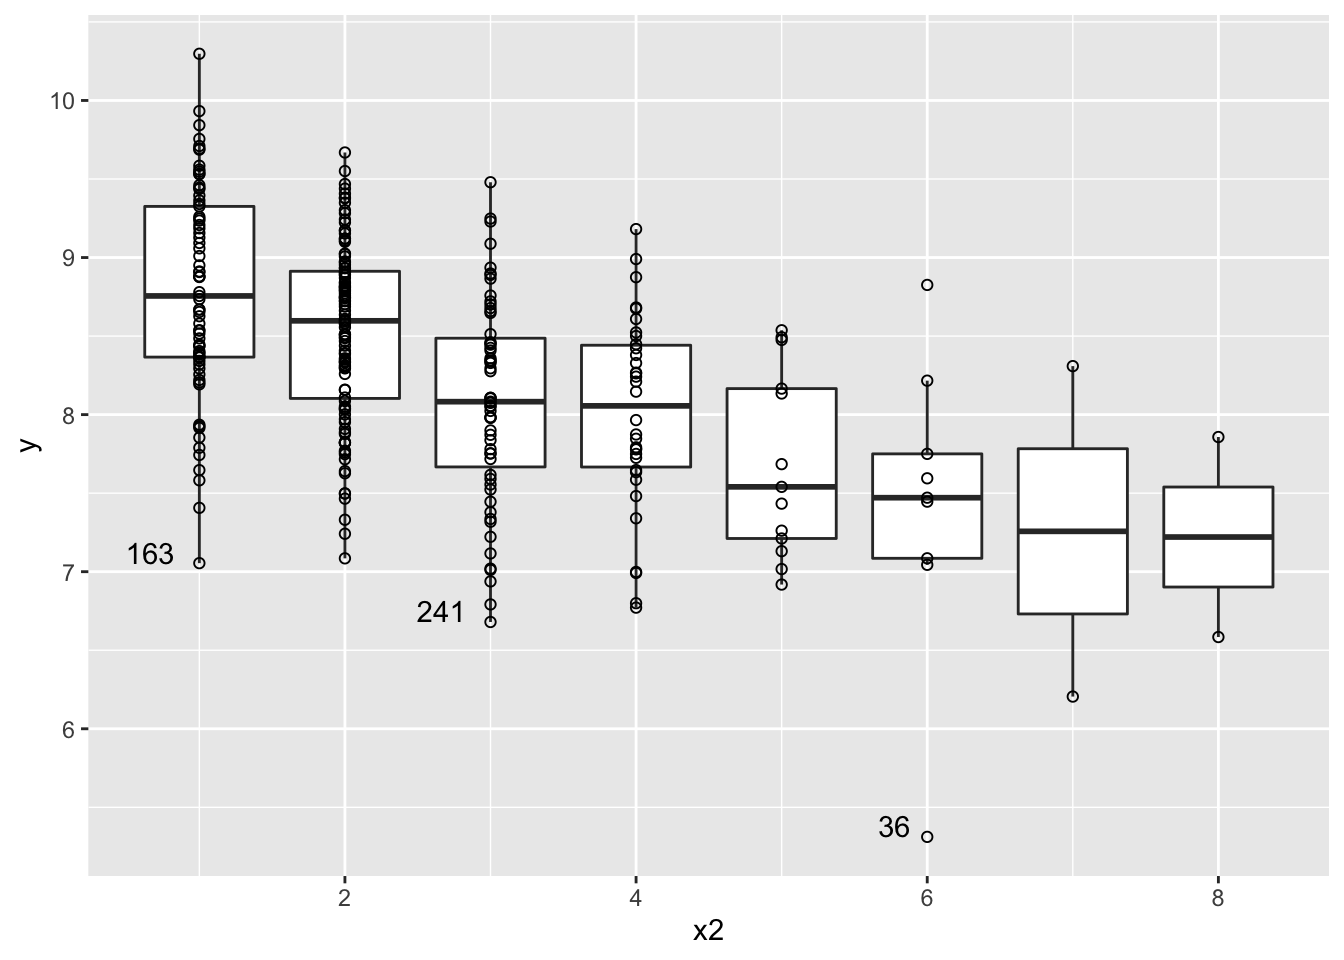
\includegraphics{main_files/figure-latex/unnamed-chunk-7-1} \end{center}

For each level of \texttt{x2} a box indicating three quantiles (25\%,
50\%, 75\%) of \texttt{y} is given. It shows that there is a tendency
for \texttt{y} to decrease with \texttt{x2} by looking at the median.
The sizes of different boxes seem to vary with different values of
\texttt{x2}. Besides, there are many observations when \texttt{x2} is
small. But it is assumed for now that the conditional variance is
constant, which will be tested section 4. Three data points with extreme
values \texttt{36}, \texttt{241} and \texttt{163} is discussed in
sections 3 and 5.

\begin{center}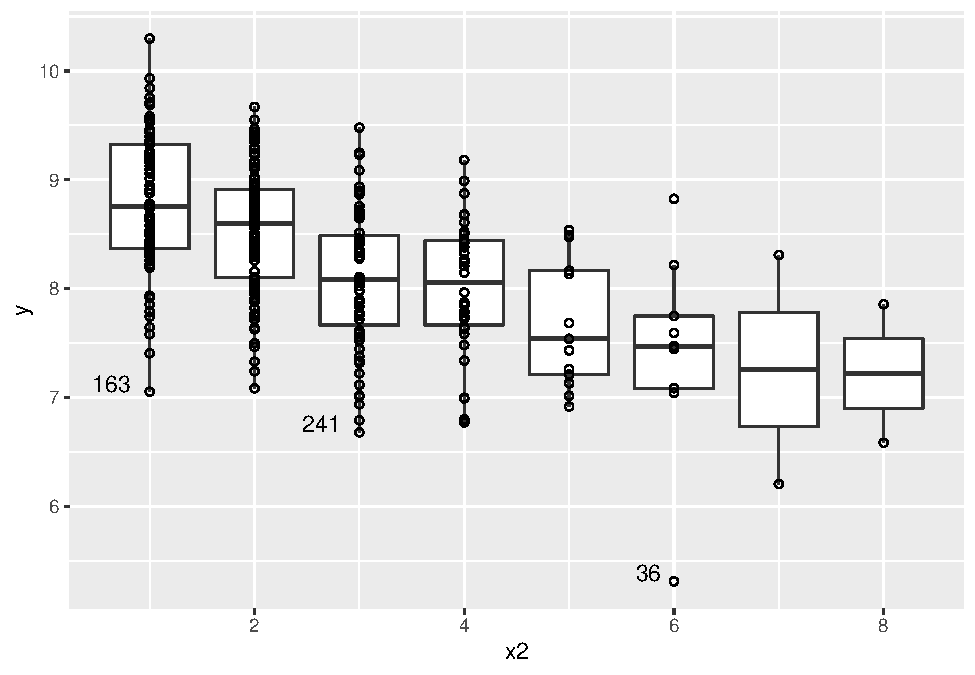
\includegraphics{main_files/figure-latex/unnamed-chunk-8-1} \end{center}

The box plot of \texttt{y} by \texttt{x6} is given. It can be seen that
the tendency is not strictly linear and the condition variance is not
stable. So we will regress \texttt{y} on \texttt{x2} first and use
\texttt{x6} as the second regressor in section 6.

\begin{center}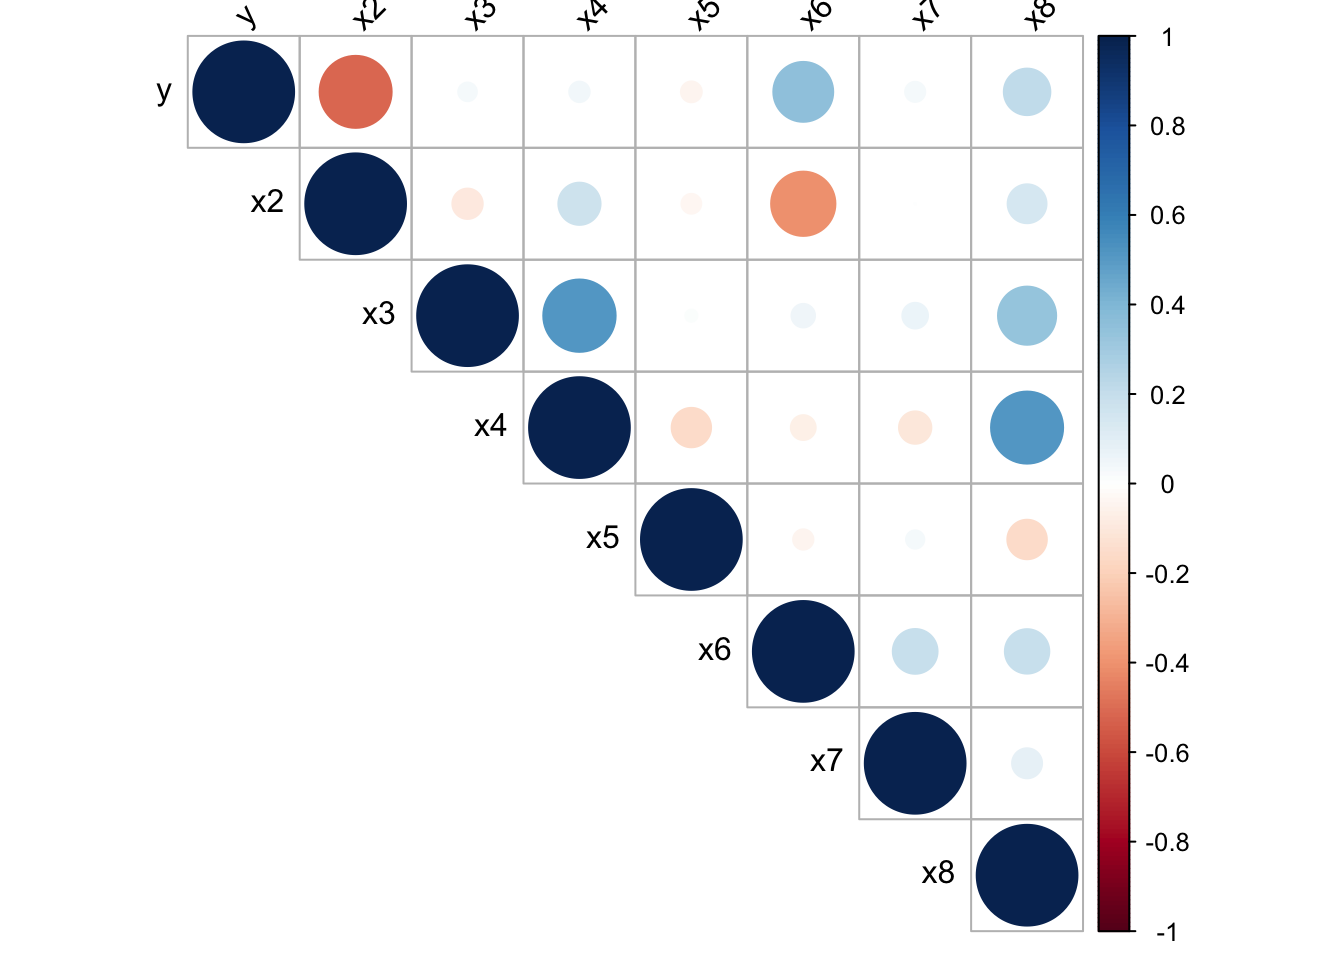
\includegraphics{main_files/figure-latex/unnamed-chunk-9-1} \end{center}

\hypertarget{regress-y-on-x2-assumptions-and-orthogonalization}{%
\subsection{\texorpdfstring{2. Regress \texttt{y} on \texttt{x2},
Assumptions and
Orthogonalization}{2. Regress y on x2, Assumptions and Orthogonalization}}\label{regress-y-on-x2-assumptions-and-orthogonalization}}

\texttt{mods{[}{[}1{]}{]}} is obtained by regressing \texttt{y} on
\texttt{x2}.

\begin{verbatim}
#> lm(formula = y ~ x2, data = dat)
\end{verbatim}

\begin{table}[H]
\centering
\begin{tabular}{lllll}
\toprule
term & estimate & std.error & statistic & p.value\\
\midrule
(Intercept) & 9.04 & 0.075 & 120 & 2.2e-254\\
x2 & -0.27 & 0.026 & -10 & 2.4e-21\\
\bottomrule
\end{tabular}
\end{table}

\begin{table}[H]
\centering
\begin{tabular}{lllllllllll}
\toprule
r.squared & adj.r.squared & sigma & statistic & p.value & df & logLik & AIC & BIC & deviance & df.residual\\
\midrule
0.26 & 0.26 & 0.63 & 105 & 2.4e-21 & 2 & -286 & 579 & 590 & 119 & 298\\
\bottomrule
\end{tabular}
\end{table}

By orthogonalizing \texttt{x2} with respect to constant 1. the following
reparameterized model can be obtained.

\begin{Shaded}
\begin{Highlighting}[]
\NormalTok{mods[[}\DecValTok{2}\NormalTok{]] <-}\StringTok{ }
\StringTok{  }\NormalTok{dat }\OperatorTok
\StringTok{  }\KeywordTok{mutate}\NormalTok{(}\DataTypeTok{x1 =} \DecValTok{1}\NormalTok{, }\DataTypeTok{x21 =}\NormalTok{ x2 }\OperatorTok{-}\StringTok{ }\KeywordTok{mean}\NormalTok{(.}\OperatorTok{$}\NormalTok{x2)) }\OperatorTok
\StringTok{  }\NormalTok{dplyr}\OperatorTok{::}\KeywordTok{select}\NormalTok{(y, x1, x21) }\OperatorTok
\StringTok{  }\NormalTok{\{}\KeywordTok{lm}\NormalTok{(y }\OperatorTok{~}\StringTok{ }\NormalTok{x1 }\OperatorTok{+}\StringTok{ }\NormalTok{x21, }\DataTypeTok{data =}\NormalTok{ .)\}}
\end{Highlighting}
\end{Shaded}

\begin{verbatim}
#> lm(formula = y ~ x1 + x21, data = .)
\end{verbatim}

\begin{table}[H]
\centering
\begin{tabular}{lllll}
\toprule
term & estimate & std.error & statistic & p.value\\
\midrule
(Intercept) & 8.36 & 0.036 & 230 & 0.0e+00\\
x21 & -0.27 & 0.026 & -10 & 2.4e-21\\
\bottomrule
\end{tabular}
\end{table}

\begin{table}[H]
\centering
\begin{tabular}{lllllllllll}
\toprule
r.squared & adj.r.squared & sigma & statistic & p.value & df & logLik & AIC & BIC & deviance & df.residual\\
\midrule
0.26 & 0.26 & 0.63 & 105 & 2.4e-21 & 2 & -286 & 579 & 590 & 119 & 298\\
\bottomrule
\end{tabular}
\end{table}

The estimated regression coefficient for \texttt{x2} in
\texttt{mods{[}{[}1{]}{]}} equals that for \texttt{x21} in
\texttt{mods{[}{[}2{]}{]}}. That is, slopes in these two models are the
same. The standard error of the intercept is reduced by 51.60 \%.

\hypertarget{normality-and-jarque-bera-test-of-mods1}{%
\subsection{\texorpdfstring{3. Normality and Jarque-Bera Test of
\texttt{mods{[}{[}1{]}{]}}}{3. Normality and Jarque-Bera Test of mods{[}{[}1{]}{]}}}\label{normality-and-jarque-bera-test-of-mods1}}

The following four plots can be used to check the plausibility of
normality assumptions:

\begin{itemize}
\tightlist
\item
  The upper left plot shows residuals against fitted values of
  \texttt{mods{[}{[}1{]}{]}}. It is hard to trust indication the flat
  trending line because there are few data points with low fitted
  values. The variance seems to be stable when fitted values are high.
  The assumption of homoskedasticity is tested formally in section 4.
\item
  Data points \texttt{36}, \texttt{241} and \texttt{163} are mentioned
  in all but the lower right plots. They are examined in section 6.
\item
  The assumption of conditional normality looks reasonable according to
  the upper right Q-Q plot. A formal Jarque-Bera test is performed later
  this section to examine this assumption in a quantitative manner.
\end{itemize}

\begin{center}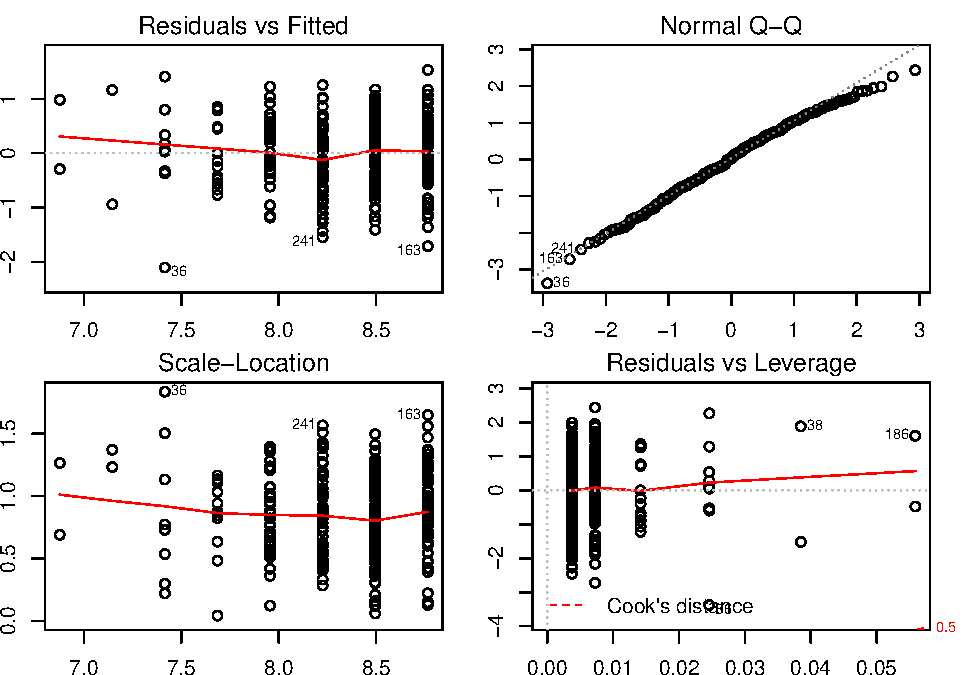
\includegraphics{main_files/figure-latex/unnamed-chunk-13-1} \end{center}

The assumption of conditional normality is justified by JB test.

\begin{table}[H]
\centering
\begin{tabular}{lllllll}
\toprule
whi & stat & df1 & df2 & p\_value & prob & if\_reject\\
\midrule
Jarque-Bera & 4.3 & 2 & 298 & 0.11 & 0.05 & FALSE\\
\bottomrule
\end{tabular}
\end{table}

Conditional distributions are visualized as follows:

\begin{verbatim}
#> `stat_bin()` using `bins = 30`. Pick better value with `binwidth`.
\end{verbatim}

\begin{center}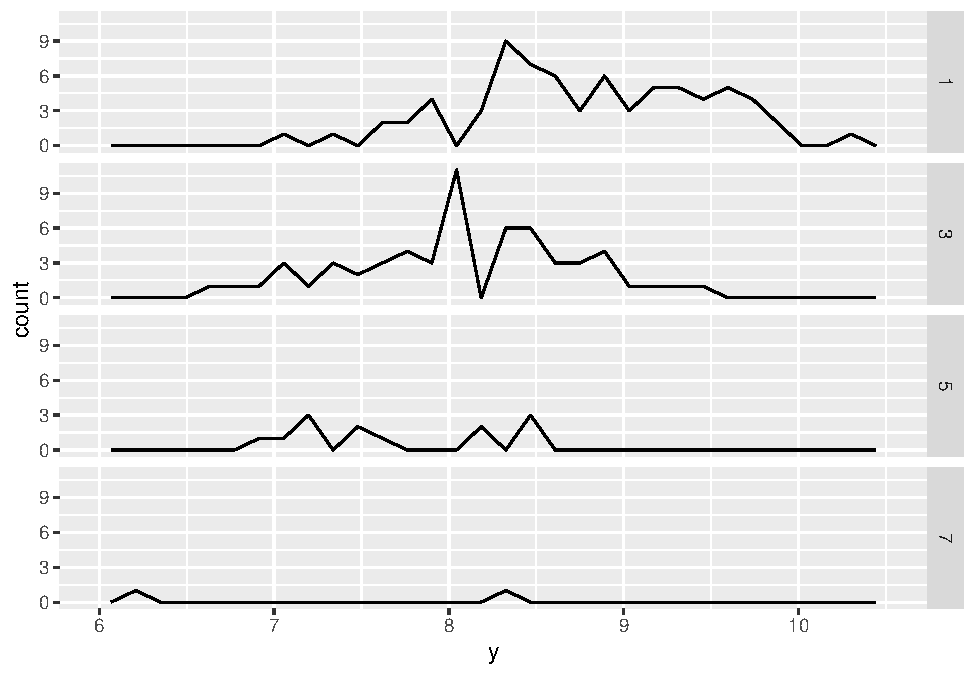
\includegraphics{main_files/figure-latex/unnamed-chunk-15-1} \end{center}

\hypertarget{homoskedasticity-and-whites-test-of-mods1}{%
\subsection{\texorpdfstring{4. Homoskedasticity and White's Test of
\texttt{mods{[}{[}1{]}{]}}}{4. Homoskedasticity and White's Test of mods{[}{[}1{]}{]}}}\label{homoskedasticity-and-whites-test-of-mods1}}

\texttt{mods{[}{[}1{]}{]}} cannot pass the White's test, which means the
variances of residuals do vary with different values of \texttt{y}.

\begin{Shaded}
\begin{Highlighting}[]
\NormalTok{mods[[}\DecValTok{1}\NormalTok{]] }\OperatorTok\StringTok{ }\KeywordTok{test_white}\NormalTok{(dat, resi2 }\OperatorTok{~}\StringTok{ }\NormalTok{x2 }\OperatorTok{+}\StringTok{ }\KeywordTok{I}\NormalTok{(x2}\OperatorTok{^}\DecValTok{2}\NormalTok{), }\DecValTok{2}\NormalTok{) }\OperatorTok\StringTok{ }\KeywordTok{tab_ti}\NormalTok{(T)}
\end{Highlighting}
\end{Shaded}

\begin{table}[H]
\centering
\begin{tabular}{lllllll}
\toprule
whi & stat & df1 & df2 & p\_value & prob & if\_reject\\
\midrule
White & 6 & 2 & 298 & 0.049 & 0.05 & TRUE\\
\bottomrule
\end{tabular}
\end{table}

\hypertarget{functional-form-and-reset-test-of-mods1}{%
\subsection{\texorpdfstring{5. Functional Form and RESET Test of
\texttt{mods{[}{[}1{]}{]}}}{5. Functional Form and RESET Test of mods{[}{[}1{]}{]}}}\label{functional-form-and-reset-test-of-mods1}}

\texttt{mods{[}{[}1{]}{]}} can pass RESET test.

\begin{table}[H]
\centering
\begin{tabular}{lllllll}
\toprule
whi & stat & df1 & df2 & p\_value & prob & if\_reject\\
\midrule
RESET & 1.1 & 1 & 299 & 0.29 & 0.05 & FALSE\\
\bottomrule
\end{tabular}
\end{table}

\hypertarget{regress-y-on-x2-with-36-data-point-excluded}{%
\subsection{\texorpdfstring{6. Regress \texttt{y} on \texttt{x2} with
\texttt{36} Data Point
Excluded}{6. Regress y on x2 with 36 Data Point Excluded}}\label{regress-y-on-x2-with-36-data-point-excluded}}

\texttt{36}, \texttt{241} and \texttt{163} data points are mentioned in
three plots regrading the analysis of residuals of
\texttt{mods{[}{[}1{]}{]}} in section 3. According to the scatter plot
in section 1, their values of \texttt{y} are too small compared to those
with same values of \texttt{x2}. They seems to be well defined.

\begin{table}[H]
\centering
\begin{tabular}{lll}
\toprule
index & y & x2\\
\midrule
36 & 5.3 & 6\\
163 & 7.1 & 1\\
241 & 6.7 & 3\\
\bottomrule
\end{tabular}
\end{table}

However, with just 8 other points when \texttt{x2} equals 6, data point
\texttt{36} will have a huge impact on the model, so it is excluded in
the following model \texttt{mods{[}{[}2{]}{]}}. That is, a new model is
estimated with the same formula as \texttt{mods{[}{[}1{]}{]}} but the
data set excluding data point \texttt{36}.

\begin{verbatim}
#> lm(formula = y ~ x2, data = .)
\end{verbatim}

\begin{table}[H]
\centering
\begin{tabular}{lllll}
\toprule
term & estimate & std.error & statistic & p.value\\
\midrule
(Intercept) & 9.01 & 0.074 & 121.3 & 5.3e-255\\
x2 & -0.26 & 0.026 & -9.8 & 6.2e-20\\
\bottomrule
\end{tabular}
\end{table}

\begin{table}[H]
\centering
\begin{tabular}{lllllllllll}
\toprule
r.squared & adj.r.squared & sigma & statistic & p.value & df & logLik & AIC & BIC & deviance & df.residual\\
\midrule
0.25 & 0.24 & 0.62 & 97 & 6.2e-20 & 2 & -280 & 566 & 577 & 114 & 297\\
\bottomrule
\end{tabular}
\end{table}

Compared with \texttt{mods{[}{[}1{]}{]}}, \texttt{mods{[}{[}2{]}{]}} has
more accurate estimation. Besides, \texttt{mods{[}{[}2{]}{]}} passes all
of the hypothesis tests. So data point \texttt{36} is exluded in the
following models, and the corresponding new data set \texttt{dat\_2} is
used.

\begin{table}[H]
\centering
\begin{tabular}{lllllll}
\toprule
whi & stat & df1 & df2 & p\_value & prob & if\_reject\\
\midrule
Jarque-Bera & 4.4 & 2 & 297 & 0.11 & 0.05 & FALSE\\
White & 1.7 & 2 & 297 & 0.43 & 0.05 & FALSE\\
RESET & 2.0 & 1 & 298 & 0.16 & 0.05 & FALSE\\
\bottomrule
\end{tabular}
\end{table}

\hypertarget{models-with-more-regressors}{%
\subsection{7. Models with More
Regressors}\label{models-with-more-regressors}}

\hypertarget{benchmark-model}{%
\subsubsection{7-1. Benchmark Model}\label{benchmark-model}}

\texttt{mods{[}{[}3{]}{]}} with \texttt{x2} and \texttt{x6} being
regressors is a good model already and pass every test. It is chosen as
the benchmark model after the discussion in subsection 7-4.

\begin{verbatim}
#> lm(formula = y ~ x2 + x6, data = dat_2)
\end{verbatim}

\begin{table}[H]
\centering
\begin{tabular}{lllll}
\toprule
term & estimate & std.error & statistic & p.value\\
\midrule
(Intercept) & 8.5222 & 0.1670 & 51.0 & 1.0e-148\\
x2 & -0.2202 & 0.0281 & -7.8 & 8.1e-14\\
x6 & 0.0076 & 0.0023 & 3.2 & 1.3e-03\\
\bottomrule
\end{tabular}
\end{table}

\begin{table}[H]
\centering
\begin{tabular}{lllllllllll}
\toprule
r.squared & adj.r.squared & sigma & statistic & p.value & df & logLik & AIC & BIC & deviance & df.residual\\
\midrule
0.27 & 0.27 & 0.61 & 55 & 4.3e-21 & 3 & -275 & 558 & 573 & 110 & 296\\
\bottomrule
\end{tabular}
\end{table}

\begin{Shaded}
\begin{Highlighting}[]
\NormalTok{results_test <-}\StringTok{ }\NormalTok{mods[[}\DecValTok{3}\NormalTok{]] }\OperatorTok\StringTok{ }\KeywordTok{test_jb}\NormalTok{(dat_}\DecValTok{2}\NormalTok{)}

\NormalTok{results_test }\OperatorTok
\StringTok{  }\KeywordTok{bind_rows}\NormalTok{(}\KeywordTok{test_white}\NormalTok{(mods[[}\DecValTok{3}\NormalTok{]], dat_}\DecValTok{2}\NormalTok{, resi2 }\OperatorTok{~}\StringTok{ }\NormalTok{x2 }\OperatorTok{+}\StringTok{ }\NormalTok{x6 }\OperatorTok{+}\StringTok{ }\KeywordTok{I}\NormalTok{(x2}\OperatorTok{^}\DecValTok{2}\NormalTok{) }\OperatorTok{+}\StringTok{ }\KeywordTok{I}\NormalTok{(x6}\OperatorTok{^}\DecValTok{2}\NormalTok{),}
    \DecValTok{3}\NormalTok{)) }\OperatorTok
\StringTok{  }\KeywordTok{bind_rows}\NormalTok{(}\KeywordTok{test_white}\NormalTok{(mods[[}\DecValTok{3}\NormalTok{]], dat_}\DecValTok{2}\NormalTok{, resi2 }\OperatorTok{~}\StringTok{ }\NormalTok{x2 }\OperatorTok{+}\StringTok{ }\NormalTok{x6 }\OperatorTok{+}\StringTok{ }\KeywordTok{I}\NormalTok{(x2}\OperatorTok{^}\DecValTok{2}\NormalTok{) }\OperatorTok{+}\StringTok{ }\KeywordTok{I}\NormalTok{(x6}\OperatorTok{^}\DecValTok{2}\NormalTok{) }\OperatorTok{+}
\StringTok{    }\KeywordTok{I}\NormalTok{(x2 }\OperatorTok{*}\StringTok{ }\NormalTok{x6), }\DecValTok{6}\NormalTok{)) }\OperatorTok
\StringTok{  }\KeywordTok{bind_rows}\NormalTok{(}\KeywordTok{test_reset}\NormalTok{(mods[[}\DecValTok{3}\NormalTok{]], dat_}\DecValTok{2}\NormalTok{))}

\NormalTok{results_test }\OperatorTok\StringTok{ }\KeywordTok{tab_ti}\NormalTok{(T)}
\end{Highlighting}
\end{Shaded}

\begin{table}[H]
\centering
\begin{tabular}{lllllll}
\toprule
whi & stat & df1 & df2 & p\_value & prob & if\_reject\\
\midrule
Jarque-Bera & 3.466 & 2 & 297 & 0.18 & 0.05 & FALSE\\
White & 1.325 & 3 & 296 & 0.72 & 0.05 & FALSE\\
White & 3.244 & 6 & 293 & 0.78 & 0.05 & FALSE\\
RESET & 0.043 & 1 & 298 & 0.84 & 0.05 & FALSE\\
\bottomrule
\end{tabular}
\end{table}

\hypertarget{model-with-all-regressors}{%
\subsubsection{7-2. Model with All
Regressors}\label{model-with-all-regressors}}

To construct \texttt{mods{[}{[}4{]}{]}}, all of the variables (excluding
\texttt{x8}) are included. \texttt{mods{[}{[}4{]}{]}} can pass
Jarque-Bera test and two White's tests, but cannot pass RESET test.

\begin{table}[H]
\centering
\begin{tabular}{llllll}
\toprule
term & estimate & std.error & statistic & p.value & p.r.squared\\
\midrule
(Intercept) & 8.6009 & 0.1975 & 43.5 & 9.9e-130 & 0.86655\\
x2 & -0.2477 & 0.0289 & -8.6 & 6.0e-16 & 0.20110\\
x3 & -0.0835 & 0.0374 & -2.2 & 2.6e-02 & 0.01683\\
x4 & 0.0621 & 0.0189 & 3.3 & 1.1e-03 & 0.03567\\
x5 & -0.0216 & 0.0710 & -0.3 & 7.6e-01 & 0.00032\\
x6 & 0.0071 & 0.0024 & 3.0 & 3.0e-03 & 0.02980\\
x7 & 0.0158 & 0.0175 & 0.9 & 3.7e-01 & 0.00278\\
\bottomrule
\end{tabular}
\end{table}

\begin{Shaded}
\begin{Highlighting}[]
\NormalTok{results_test <-}\StringTok{ }\NormalTok{mods[[}\DecValTok{4}\NormalTok{]] }\OperatorTok\StringTok{ }\KeywordTok{test_jb}\NormalTok{(dat_}\DecValTok{2}\NormalTok{)}

\NormalTok{results_test }\OperatorTok
\StringTok{  }\KeywordTok{bind_rows}\NormalTok{(}\KeywordTok{test_white}\NormalTok{(mods[[}\DecValTok{4}\NormalTok{]], dat_}\DecValTok{2}\NormalTok{, resi2 }\OperatorTok{~}\StringTok{ }\NormalTok{x2 }\OperatorTok{+}\StringTok{ }\NormalTok{x3 }\OperatorTok{+}\StringTok{ }\NormalTok{x4 }\OperatorTok{+}\StringTok{ }\NormalTok{x5 }\OperatorTok{+}\StringTok{ }\NormalTok{x6 }\OperatorTok{+}\StringTok{ }\NormalTok{x7 }\OperatorTok{+}\StringTok{ }
\StringTok{    }\KeywordTok{I}\NormalTok{(x2}\OperatorTok{^}\DecValTok{2}\NormalTok{) }\OperatorTok{+}\StringTok{ }\KeywordTok{I}\NormalTok{(x3}\OperatorTok{^}\DecValTok{2}\NormalTok{) }\OperatorTok{+}\StringTok{ }\KeywordTok{I}\NormalTok{(x4}\OperatorTok{^}\DecValTok{2}\NormalTok{) }\OperatorTok{+}\StringTok{ }\KeywordTok{I}\NormalTok{(x5}\OperatorTok{^}\DecValTok{2}\NormalTok{) }\OperatorTok{+}\StringTok{ }\KeywordTok{I}\NormalTok{(x6}\OperatorTok{^}\DecValTok{2}\NormalTok{) }\OperatorTok{+}\StringTok{ }\KeywordTok{I}\NormalTok{(x7}\OperatorTok{^}\DecValTok{2}\NormalTok{), }\DecValTok{7}\NormalTok{)) }\OperatorTok
\StringTok{  }\KeywordTok{bind_rows}\NormalTok{(}\KeywordTok{test_white}\NormalTok{(mods[[}\DecValTok{4}\NormalTok{]], dat_}\DecValTok{2}\NormalTok{, resi2 }\OperatorTok{~}\StringTok{ }\NormalTok{x2 }\OperatorTok{+}\StringTok{ }\NormalTok{x3 }\OperatorTok{+}\StringTok{ }\NormalTok{x4 }\OperatorTok{+}\StringTok{ }\NormalTok{x5 }\OperatorTok{+}\StringTok{ }\NormalTok{x6 }\OperatorTok{+}\StringTok{ }\NormalTok{x7 }\OperatorTok{+}\StringTok{ }
\StringTok{    }\KeywordTok{I}\NormalTok{(x2}\OperatorTok{^}\DecValTok{2}\NormalTok{) }\OperatorTok{+}\StringTok{ }\KeywordTok{I}\NormalTok{(x3}\OperatorTok{^}\DecValTok{2}\NormalTok{) }\OperatorTok{+}\StringTok{ }\KeywordTok{I}\NormalTok{(x4}\OperatorTok{^}\DecValTok{2}\NormalTok{) }\OperatorTok{+}\StringTok{ }\KeywordTok{I}\NormalTok{(x5}\OperatorTok{^}\DecValTok{2}\NormalTok{) }\OperatorTok{+}\StringTok{ }\KeywordTok{I}\NormalTok{(x6}\OperatorTok{^}\DecValTok{2}\NormalTok{) }\OperatorTok{+}\StringTok{ }\KeywordTok{I}\NormalTok{(x7}\OperatorTok{^}\DecValTok{2}\NormalTok{) }\OperatorTok{+}\StringTok{ }\KeywordTok{I}\NormalTok{(x2 }\OperatorTok{*}\StringTok{ }\NormalTok{x3) }\OperatorTok{+}
\StringTok{    }\KeywordTok{I}\NormalTok{(x2 }\OperatorTok{*}\StringTok{ }\NormalTok{x4) }\OperatorTok{+}\StringTok{ }\KeywordTok{I}\NormalTok{(x2 }\OperatorTok{*}\StringTok{ }\NormalTok{x5) }\OperatorTok{+}\StringTok{ }\KeywordTok{I}\NormalTok{(x2 }\OperatorTok{*}\StringTok{ }\NormalTok{x6) }\OperatorTok{+}\StringTok{ }\KeywordTok{I}\NormalTok{(x2 }\OperatorTok{*}\StringTok{ }\NormalTok{x7) }\OperatorTok{+}\StringTok{ }\KeywordTok{I}\NormalTok{(x4 }\OperatorTok{*}\StringTok{ }\NormalTok{x3) }\OperatorTok{+}\StringTok{ }
\StringTok{    }\KeywordTok{I}\NormalTok{(x5 }\OperatorTok{*}\StringTok{ }\NormalTok{x3) }\OperatorTok{+}\StringTok{ }\KeywordTok{I}\NormalTok{(x6 }\OperatorTok{*}\StringTok{ }\NormalTok{x3) }\OperatorTok{+}\StringTok{ }\KeywordTok{I}\NormalTok{(x3 }\OperatorTok{*}\StringTok{ }\NormalTok{x7) }\OperatorTok{+}\StringTok{ }\KeywordTok{I}\NormalTok{(x4 }\OperatorTok{*}\StringTok{ }\NormalTok{x5) }\OperatorTok{+}\StringTok{ }\KeywordTok{I}\NormalTok{(x4 }\OperatorTok{*}\StringTok{ }\NormalTok{x6) }\OperatorTok{+}\StringTok{ }
\StringTok{    }\KeywordTok{I}\NormalTok{(x4 }\OperatorTok{*}\StringTok{ }\NormalTok{x7) }\OperatorTok{+}\StringTok{ }\KeywordTok{I}\NormalTok{(x5 }\OperatorTok{*}\StringTok{ }\NormalTok{x6) }\OperatorTok{+}\StringTok{ }\KeywordTok{I}\NormalTok{(x5 }\OperatorTok{*}\StringTok{ }\NormalTok{x7) }\OperatorTok{+}\StringTok{ }\KeywordTok{I}\NormalTok{(x6 }\OperatorTok{*}\StringTok{ }\NormalTok{x7), }\DecValTok{28}\NormalTok{)) }\OperatorTok
\StringTok{  }\KeywordTok{bind_rows}\NormalTok{(}\KeywordTok{test_reset}\NormalTok{(mods[[}\DecValTok{4}\NormalTok{]], dat_}\DecValTok{2}\NormalTok{))}

\NormalTok{results_test }\OperatorTok\StringTok{ }\KeywordTok{tab_ti}\NormalTok{(T)}
\end{Highlighting}
\end{Shaded}

\begin{table}[H]
\centering
\begin{tabular}{lllllll}
\toprule
whi & stat & df1 & df2 & p\_value & prob & if\_reject\\
\midrule
Jarque-Bera & 1.8 & 2 & 297 & 0.406 & 0.05 & FALSE\\
White & 12.3 & 7 & 292 & 0.090 & 0.05 & FALSE\\
White & 31.0 & 28 & 271 & 0.316 & 0.05 & FALSE\\
RESET & 4.1 & 1 & 298 & 0.043 & 0.05 & TRUE\\
\bottomrule
\end{tabular}
\end{table}

\hypertarget{likelihood-ratio-test}{%
\subsubsection{7-3. Likelihood Ratio Test}\label{likelihood-ratio-test}}

Likelihood ratio tests for restricting one parameter can be performed by
using partial correlations. For example, to test the hypothesis that
coefficient for \texttt{x5} is 0 in \texttt{mods{[}{[}4{]}{]}},
following calculation can be conducted. With \texttt{p\_value} being
0.7581638, we cannot reject the hypothesis.

\begin{Shaded}
\begin{Highlighting}[]
\NormalTok{lr_x5 <-}\StringTok{ }\OperatorTok{-}\StringTok{ }\DecValTok{299} \OperatorTok{*}\StringTok{ }\KeywordTok{log}\NormalTok{(}\DecValTok{1} \OperatorTok{-}\StringTok{ }\FloatTok{0.0003170}\NormalTok{) }
\NormalTok{(}\DecValTok{1} \OperatorTok{-}\StringTok{ }\KeywordTok{pchisq}\NormalTok{(lr_x5, }\DecValTok{1}\NormalTok{))}
\end{Highlighting}
\end{Shaded}

\begin{verbatim}
#> [1] 0.7581638
\end{verbatim}

\begin{table}[H]
\centering
\begin{tabular}{lllllll}
\toprule
whi & stat & df1 & df2 & p\_value & prob & if\_reject\\
\midrule
logLik & 0.095 & 1 & 299 & 0.76 & 0.05 & FALSE\\
\bottomrule
\end{tabular}
\end{table}

Likelihood tests for restricting more than one parameter can be only
performed by using values of log likelihood in the original and
restricted models. For example, to test the hypothesis that coefficients
for \texttt{x5} and \texttt{x7} are both 0 in
\texttt{mods{[}{[}4{]}{]}}, following calculation can be conducted. We
cannot reject the hypothesis according the function output.

\begin{table}[H]
\centering
\begin{tabular}{lllllll}
\toprule
whi & stat & df1 & df2 & p\_value & prob & if\_reject\\
\midrule
logLik & 0.92 & 2 & 298 & 0.34 & 0.05 & FALSE\\
\bottomrule
\end{tabular}
\end{table}

\begin{table}[H]
\centering
\begin{tabular}{lllllll}
\toprule
whi & stat & df1 & df2 & p\_value & prob & if\_reject\\
\midrule
logLik & 0.82 & 1 & 299 & 0.36 & 0.05 & FALSE\\
\bottomrule
\end{tabular}
\end{table}

The above three test statistics are related in an additive manner, so
models with multiple regressors can be reduced in a step-wise procedure.
During every step, partial correlations for regressors can be used as
the indication of the next term to be reduced.

\begin{verbatim}
#> [1] TRUE
\end{verbatim}

\hypertarget{automated-model-selection}{%
\subsubsection{7-4. Automated Model
Selection}\label{automated-model-selection}}

Thus, \texttt{mods{[}{[}5{]}{]}} is determined by automated model
selection using \texttt{mods{[}{[}4{]}{]}} with \texttt{stats::step}
function. \texttt{mods{[}{[}5{]}{]}} can pass Jarque-Bera test and two
White's tests, but cannot pass RESET test.

\begin{verbatim}
#> lm(formula = y ~ x2 + x3 + x4 + x6, data = dat_2)
\end{verbatim}

\begin{table}[H]
\centering
\begin{tabular}{lllll}
\toprule
term & estimate & std.error & statistic & p.value\\
\midrule
(Intercept) & 8.6023 & 0.1914 & 44.9 & 1.0e-133\\
x2 & -0.2442 & 0.0286 & -8.5 & 7.4e-16\\
x3 & -0.0799 & 0.0367 & -2.2 & 3.0e-02\\
x4 & 0.0603 & 0.0183 & 3.3 & 1.1e-03\\
x6 & 0.0076 & 0.0023 & 3.3 & 1.1e-03\\
\bottomrule
\end{tabular}
\end{table}

\begin{table}[H]
\centering
\begin{tabular}{lllllllllll}
\toprule
r.squared & adj.r.squared & sigma & statistic & p.value & df & logLik & AIC & BIC & deviance & df.residual\\
\midrule
0.3 & 0.29 & 0.6 & 31 & 1.2e-21 & 5 & -269 & 551 & 573 & 106 & 294\\
\bottomrule
\end{tabular}
\end{table}

\begin{Shaded}
\begin{Highlighting}[]
\NormalTok{results_test <-}\StringTok{ }\NormalTok{mods[[}\DecValTok{5}\NormalTok{]] }\OperatorTok\StringTok{ }\KeywordTok{test_jb}\NormalTok{(dat_}\DecValTok{2}\NormalTok{)}

\NormalTok{results_test }\OperatorTok
\StringTok{  }\KeywordTok{bind_rows}\NormalTok{(}\KeywordTok{test_white}\NormalTok{(mods[[}\DecValTok{5}\NormalTok{]], dat_}\DecValTok{2}\NormalTok{, resi2 }\OperatorTok{~}\StringTok{ }\NormalTok{x2 }\OperatorTok{+}\StringTok{ }\NormalTok{x3 }\OperatorTok{+}\StringTok{ }\NormalTok{x4 }\OperatorTok{+}\StringTok{ }\NormalTok{x6 }\OperatorTok{+}\StringTok{ }\KeywordTok{I}\NormalTok{(x2}\OperatorTok{^}\DecValTok{2}\NormalTok{) }\OperatorTok{+}
\StringTok{    }\KeywordTok{I}\NormalTok{(x3}\OperatorTok{^}\DecValTok{2}\NormalTok{) }\OperatorTok{+}\StringTok{ }\KeywordTok{I}\NormalTok{(x4}\OperatorTok{^}\DecValTok{2}\NormalTok{) }\OperatorTok{+}\StringTok{ }\KeywordTok{I}\NormalTok{(x6}\OperatorTok{^}\DecValTok{2}\NormalTok{), }\DecValTok{5}\NormalTok{)) }\OperatorTok
\StringTok{  }\KeywordTok{bind_rows}\NormalTok{(}\KeywordTok{test_white}\NormalTok{(mods[[}\DecValTok{5}\NormalTok{]], dat_}\DecValTok{2}\NormalTok{, resi2 }\OperatorTok{~}\StringTok{ }\NormalTok{x2 }\OperatorTok{+}\StringTok{ }\NormalTok{x3 }\OperatorTok{+}\StringTok{ }\NormalTok{x4 }\OperatorTok{+}\StringTok{ }\NormalTok{x6 }\OperatorTok{+}\StringTok{ }
\StringTok{    }\KeywordTok{I}\NormalTok{(x2}\OperatorTok{^}\DecValTok{2}\NormalTok{) }\OperatorTok{+}\StringTok{ }\KeywordTok{I}\NormalTok{(x3}\OperatorTok{^}\DecValTok{2}\NormalTok{) }\OperatorTok{+}\StringTok{ }\KeywordTok{I}\NormalTok{(x4}\OperatorTok{^}\DecValTok{2}\NormalTok{) }\OperatorTok{+}\StringTok{ }\KeywordTok{I}\NormalTok{(x6}\OperatorTok{^}\DecValTok{2}\NormalTok{) }\OperatorTok{+}\StringTok{ }\KeywordTok{I}\NormalTok{(x2 }\OperatorTok{*}\StringTok{ }\NormalTok{x3) }\OperatorTok{+}\StringTok{ }\KeywordTok{I}\NormalTok{(x2 }\OperatorTok{*}\StringTok{ }\NormalTok{x4) }\OperatorTok{+}\StringTok{ }
\StringTok{    }\KeywordTok{I}\NormalTok{(x2 }\OperatorTok{*}\StringTok{ }\NormalTok{x6) }\OperatorTok{+}\StringTok{ }\KeywordTok{I}\NormalTok{(x4 }\OperatorTok{*}\StringTok{ }\NormalTok{x3) }\OperatorTok{+}\StringTok{ }\KeywordTok{I}\NormalTok{(x6 }\OperatorTok{*}\StringTok{ }\NormalTok{x3) }\OperatorTok{+}\KeywordTok{I}\NormalTok{(x4 }\OperatorTok{*}\StringTok{ }\NormalTok{x6), }\DecValTok{15}\NormalTok{)) }\OperatorTok
\StringTok{  }\KeywordTok{bind_rows}\NormalTok{(}\KeywordTok{test_reset}\NormalTok{(mods[[}\DecValTok{5}\NormalTok{]], dat_}\DecValTok{2}\NormalTok{))}

\NormalTok{results_test }\OperatorTok\StringTok{ }\KeywordTok{tab_ti}\NormalTok{(T)}
\end{Highlighting}
\end{Shaded}

\begin{table}[H]
\centering
\begin{tabular}{lllllll}
\toprule
whi & stat & df1 & df2 & p\_value & prob & if\_reject\\
\midrule
Jarque-Bera & 2.0 & 2 & 297 & 0.371 & 0.05 & FALSE\\
White & 10.1 & 5 & 294 & 0.074 & 0.05 & FALSE\\
White & 19.4 & 15 & 284 & 0.197 & 0.05 & FALSE\\
RESET & 3.9 & 1 & 298 & 0.048 & 0.05 & TRUE\\
\bottomrule
\end{tabular}
\end{table}

According to results of five models, though \texttt{mods{[}{[}4{]}{]}}
and \texttt{mods{[}{[}5{]}{]}} have lower AIC,
\texttt{mods{[}{[}3{]}{]}} is the one with all tests passed and lowst
AIC. It is discussed intensively in subsection 8-1, and acts as the
benchmark model in section 9. Besides, \texttt{mods{[}{[}3{]}{]}} has
the lowest BIC.

\begin{table}[H]
\centering
\begin{tabular}{llllllllllll}
\toprule
index & r.squared & adj.r.squared & sigma & statistic & p.value & df & logLik & AIC & BIC & deviance & df.residual\\
\midrule
1 & 0.26 & 0.26 & 0.63 & 105 & 2.4e-21 & 2 & -286 & 579 & 590 & 119 & 298\\
2 & 0.26 & 0.26 & 0.63 & 105 & 2.4e-21 & 2 & -286 & 579 & 590 & 119 & 298\\
3 & 0.27 & 0.27 & 0.61 & 55 & 4.3e-21 & 3 & -275 & 558 & 573 & 110 & 296\\
4 & 0.30 & 0.29 & 0.60 & 21 & 2.4e-20 & 7 & -269 & 554 & 584 & 106 & 292\\
5 & 0.30 & 0.29 & 0.60 & 31 & 1.2e-21 & 5 & -269 & 551 & 573 & 106 & 294\\
\bottomrule
\end{tabular}
\end{table}

Additionally, \texttt{mods{[}{[}4{]}{]}} has the highest
\texttt{r.squared} for including more regressors, but its
\texttt{adj.r.squared} is penalized for that. The AIC and BIC are not
low as well compared to those of \texttt{mods{[}{[}3{]}{]}} and
\texttt{mods{[}{[}5{]}{]}}.

\hypertarget{causality-and-mediation}{%
\subsection{8. Causality and Mediation}\label{causality-and-mediation}}

\hypertarget{causality-of-x2-x6}{%
\subsubsection{\texorpdfstring{8-1. Causality of
\texttt{x2}-\texttt{x6}}{8-1. Causality of x2-x6}}\label{causality-of-x2-x6}}

It can be seen from the following two models that \texttt{y} is highly
correlated to \texttt{x2} and \texttt{x6} separately. Besides, according
to \texttt{mods{[}{[}3{]}{]}}, \texttt{y} is highly correlated to
\texttt{x2} and \texttt{x6} at the same time.

\begin{verbatim}
#> lm(formula = y ~ x2, data = dat_2)
\end{verbatim}

\begin{table}[H]
\centering
\begin{tabular}{lllll}
\toprule
term & estimate & std.error & statistic & p.value\\
\midrule
(Intercept) & 9.01 & 0.074 & 121.3 & 5.3e-255\\
x2 & -0.26 & 0.026 & -9.8 & 6.2e-20\\
\bottomrule
\end{tabular}
\end{table}

\begin{table}[H]
\centering
\begin{tabular}{lllllllllll}
\toprule
r.squared & adj.r.squared & sigma & statistic & p.value & df & logLik & AIC & BIC & deviance & df.residual\\
\midrule
0.25 & 0.24 & 0.62 & 97 & 6.2e-20 & 2 & -280 & 566 & 577 & 114 & 297\\
\bottomrule
\end{tabular}
\end{table}

\begin{verbatim}
#> lm(formula = y ~ x6, data = dat_2)
\end{verbatim}

\begin{table}[H]
\centering
\begin{tabular}{lllll}
\toprule
term & estimate & std.error & statistic & p.value\\
\midrule
(Intercept) & 7.589 & 0.1286 & 59.0 & 4.1e-166\\
x6 & 0.015 & 0.0023 & 6.4 & 7.2e-10\\
\bottomrule
\end{tabular}
\end{table}

\begin{table}[H]
\centering
\begin{tabular}{lllllllllll}
\toprule
r.squared & adj.r.squared & sigma & statistic & p.value & df & logLik & AIC & BIC & deviance & df.residual\\
\midrule
0.12 & 0.12 & 0.67 & 41 & 7.2e-10 & 2 & -303 & 612 & 623 & 133 & 297\\
\bottomrule
\end{tabular}
\end{table}

It is reasonable to assume that people tend to have more accompanies as
age increases after 18. Also, the following model proves the
relationship between \texttt{x2} and \texttt{x6}. We can say that the
effect of \texttt{x6} on \texttt{y} is mediated by \texttt{x2}. With
\texttt{x6} affecting \texttt{y} as well, \texttt{x2} does not mediate
\texttt{x6} completely. So \texttt{x2} and \texttt{x6} are both supposed
to appear in the model for \texttt{y}. The mediation factor \texttt{x2}
may affect \texttt{y} though other ways, which will be explored in
section 10. Besides, we find that \texttt{x6} does not affect \texttt{y}
in other ways in section 10.

\begin{verbatim}
#> lm(formula = x2 ~ x6, data = dat_2)
\end{verbatim}

\begin{table}[H]
\centering
\begin{tabular}{lllll}
\toprule
term & estimate & std.error & statistic & p.value\\
\midrule
(Intercept) & 4.238 & 0.2422 & 17.5 & 1.3e-47\\
x6 & -0.033 & 0.0044 & -7.6 & 5.1e-13\\
\bottomrule
\end{tabular}
\end{table}

\begin{table}[H]
\centering
\begin{tabular}{lllllllllll}
\toprule
r.squared & adj.r.squared & sigma & statistic & p.value & df & logLik & AIC & BIC & deviance & df.residual\\
\midrule
0.16 & 0.16 & 1.3 & 57 & 5.1e-13 & 2 & -492 & 991 & 1002 & 472 & 297\\
\bottomrule
\end{tabular}
\end{table}

\hypertarget{causality-of-x3-x4}{%
\subsubsection{\texorpdfstring{8-2. Causality of
\texttt{x3}-\texttt{x4}}{8-2. Causality of x3-x4}}\label{causality-of-x3-x4}}

When taking \texttt{x3} and \texttt{x4} into consideration, the models
assocating \texttt{y} with \texttt{x3} or \texttt{x4} both show no
significance, though \texttt{x3} and \texttt{x4} are highly correlated.
So neither \texttt{x3} nor \texttt{x4} should be included in the model.

\begin{verbatim}
#> lm(formula = x4 ~ x3, data = dat_2)
\end{verbatim}

\begin{table}[H]
\centering
\begin{tabular}{lllll}
\toprule
term & estimate & std.error & statistic & p.value\\
\midrule
(Intercept) & 0.51 & 0.33 & 1.5 & 1.2e-01\\
x3 & 1.05 & 0.10 & 10.3 & 1.3e-21\\
\bottomrule
\end{tabular}
\end{table}

\begin{table}[H]
\centering
\begin{tabular}{lllllllllll}
\toprule
r.squared & adj.r.squared & sigma & statistic & p.value & df & logLik & AIC & BIC & deviance & df.residual\\
\midrule
0.26 & 0.26 & 2 & 107 & 1.3e-21 & 2 & -627 & 1260 & 1271 & 1161 & 297\\
\bottomrule
\end{tabular}
\end{table}

\begin{verbatim}
#> lm(formula = y ~ x3 + x4, data = dat_2)
\end{verbatim}

\begin{table}[H]
\centering
\begin{tabular}{lllll}
\toprule
term & estimate & std.error & statistic & p.value\\
\midrule
(Intercept) & 8.3240 & 0.120 & 69.30 & 5.3e-185\\
x3 & 0.0046 & 0.043 & 0.11 & 9.1e-01\\
x4 & 0.0086 & 0.021 & 0.41 & 6.8e-01\\
\bottomrule
\end{tabular}
\end{table}

\begin{table}[H]
\centering
\begin{tabular}{lllllllllll}
\toprule
r.squared & adj.r.squared & sigma & statistic & p.value & df & logLik & AIC & BIC & deviance & df.residual\\
\midrule
0.001 & -0.0057 & 0.71 & 0.15 & 0.86 & 3 & -322 & 652 & 667 & 151 & 296\\
\bottomrule
\end{tabular}
\end{table}

\hypertarget{causality-of-x4-x8}{%
\subsubsection{\texorpdfstring{8-3. Causality of
\texttt{x4}-\texttt{x8}}{8-3. Causality of x4-x8}}\label{causality-of-x4-x8}}

It can be seen that \texttt{y} is highly correlated to \texttt{x8}.

\begin{verbatim}
#> lm(formula = y ~ x8, data = dat_2)
\end{verbatim}

\begin{table}[H]
\centering
\begin{tabular}{lllll}
\toprule
term & estimate & std.error & statistic & p.value\\
\midrule
(Intercept) & 7.993 & 0.114 & 70.2 & 6.7e-187\\
x8 & 0.046 & 0.013 & 3.5 & 4.7e-04\\
\bottomrule
\end{tabular}
\end{table}

\begin{table}[H]
\centering
\begin{tabular}{lllllllllll}
\toprule
r.squared & adj.r.squared & sigma & statistic & p.value & df & logLik & AIC & BIC & deviance & df.residual\\
\midrule
0.04 & 0.037 & 0.7 & 13 & 0.00047 & 2 & -316 & 638 & 649 & 145 & 297\\
\bottomrule
\end{tabular}
\end{table}

Also, \texttt{x8} is highly related to \texttt{x4}, which makes sense,
because people with more income tend to buy houses with more rooms.

\begin{verbatim}
#> lm(formula = x8 ~ x4, data = dat_2)
\end{verbatim}

\begin{table}[H]
\centering
\begin{tabular}{lllll}
\toprule
term & estimate & std.error & statistic & p.value\\
\midrule
(Intercept) & 5.62 & 0.295 & 19 & 2.5e-53\\
x4 & 0.69 & 0.067 & 10 & 3.1e-21\\
\bottomrule
\end{tabular}
\end{table}

\begin{table}[H]
\centering
\begin{tabular}{lllllllllll}
\toprule
r.squared & adj.r.squared & sigma & statistic & p.value & df & logLik & AIC & BIC & deviance & df.residual\\
\midrule
0.26 & 0.26 & 2.7 & 105 & 3.1e-21 & 2 & -718 & 1442 & 1453 & 2132 & 297\\
\bottomrule
\end{tabular}
\end{table}

However, from subsection 9.2 we already know that \texttt{y} is not
highly correlated with \texttt{x4}, which is illustrated again by the
following model. So we say that the effect of \texttt{x4} on \texttt{y}
is completely mediated by \texttt{x8}. Though it makes sense that people
with more income tend to consume more energy on average, the direct
effect is completely mediated through \texttt{x8} and possibly other
factors.

\begin{verbatim}
#> lm(formula = y ~ x8 + x4, data = dat_2)
\end{verbatim}

\begin{table}[H]
\centering
\begin{tabular}{lllll}
\toprule
term & estimate & std.error & statistic & p.value\\
\midrule
(Intercept) & 8.012 & 0.114 & 70.0 & 3.2e-186\\
x8 & 0.057 & 0.015 & 3.8 & 1.8e-04\\
x4 & -0.030 & 0.020 & -1.5 & 1.5e-01\\
\bottomrule
\end{tabular}
\end{table}

\begin{table}[H]
\centering
\begin{tabular}{lllllllllll}
\toprule
r.squared & adj.r.squared & sigma & statistic & p.value & df & logLik & AIC & BIC & deviance & df.residual\\
\midrule
0.047 & 0.041 & 0.7 & 7.3 & 0.00077 & 3 & -315 & 638 & 653 & 144 & 296\\
\bottomrule
\end{tabular}
\end{table}

\hypertarget{mods3-with-extra-terms}{%
\subsection{\texorpdfstring{9. \texttt{mods{[}{[}3{]}{]}} with extra
terms}{9. mods{[}{[}3{]}{]} with extra terms}}\label{mods3-with-extra-terms}}

In \texttt{mods{[}{[}6{]}{]}}, \texttt{x2}, \texttt{x6} and \texttt{x8}
are kept at the same time.

\begin{verbatim}
#> lm(formula = y ~ x2 + x6 + x8, data = dat_2)
\end{verbatim}

\begin{table}[H]
\centering
\begin{tabular}{lllll}
\toprule
term & estimate & std.error & statistic & p.value\\
\midrule
(Intercept) & 8.3053 & 0.1652 & 50.3 & 1.0e-146\\
x2 & -0.2592 & 0.0279 & -9.3 & 3.5e-18\\
x6 & 0.0041 & 0.0023 & 1.8 & 7.8e-02\\
x8 & 0.0605 & 0.0115 & 5.3 & 2.7e-07\\
\bottomrule
\end{tabular}
\end{table}

\begin{table}[H]
\centering
\begin{tabular}{lllllllllll}
\toprule
r.squared & adj.r.squared & sigma & statistic & p.value & df & logLik & AIC & BIC & deviance & df.residual\\
\midrule
0.33 & 0.33 & 0.58 & 49 & 7.2e-26 & 4 & -262 & 533 & 552 & 101 & 295\\
\bottomrule
\end{tabular}
\end{table}

\begin{table}[H]
\centering
\begin{tabular}{lllllll}
\toprule
whi & stat & df1 & df2 & p\_value & prob & if\_reject\\
\midrule
Jarque-Bera & 2.9 & 2 & 297 & 0.24 & 0.05 & FALSE\\
White & 3.9 & 4 & 295 & 0.42 & 0.05 & FALSE\\
White & 9.7 & 10 & 289 & 0.46 & 0.05 & FALSE\\
RESET & 2.1 & 1 & 298 & 0.15 & 0.05 & FALSE\\
\bottomrule
\end{tabular}
\end{table}

With the idea of diminishing effects of the number of household members
in mind, it is natural to include the square of the household numbers.
In addition, \texttt{x8} is included according to the discussion in
subsection 8-3. Thus, \texttt{mods{[}{[}7{]}{]}} is estimated. Being
insignificant, \texttt{x6} is excluded, beccause the effect of
\texttt{x6} on \texttt{y} seems to be mediated compeletely by
\texttt{x2} and \texttt{x2\^{}2}.

\begin{table}[H]
\centering
\begin{tabular}{llllll}
\toprule
term & estimate & std.error & statistic & p.value & p.r.squared\\
\midrule
(Intercept) & 8.779 & 0.137 & 64.3 & 1.5e-175 & 0.933\\
x2 & -0.521 & 0.086 & -6.0 & 5.0e-09 & 0.110\\
x8 & 0.073 & 0.011 & 6.5 & 2.6e-10 & 0.127\\
I(x2\textasciicircum{}2) & 0.036 & 0.012 & 2.9 & 4.1e-03 & 0.028\\
\bottomrule
\end{tabular}
\end{table}

With number of observations being 299, the model is sensitive to
exlusion of some term only if the partial correlation of that term is
smaller than 0.01276551. That is, if \texttt{p.r.squared} of some term
displayed above is smaller than 0.01276551, the hypothesis regaring the
coefficient for that term in the likelihood ratio test would not be
rejected. The value \texttt{0.01276551} is obtained according to the
discussion in subsection 7-3. Besides, small \texttt{p.value}s indicate
that terms cannot be excluded as well.

\begin{table}[H]
\centering
\begin{tabular}{lllllll}
\toprule
whi & stat & df1 & df2 & p\_value & prob & if\_reject\\
\midrule
Jarque-Bera & 3.934 & 2 & 297 & 0.14 & 0.05 & FALSE\\
White & 2.289 & 3 & 296 & 0.51 & 0.05 & FALSE\\
White & 2.364 & 6 & 293 & 0.88 & 0.05 & FALSE\\
RESET & 0.068 & 1 & 298 & 0.79 & 0.05 & FALSE\\
\bottomrule
\end{tabular}
\end{table}

\texttt{mods{[}{[}7{]}{]}} has a lower AIC than
\texttt{mods{[}{[}6{]}{]}} and \texttt{mods{[}{[}3{]}{]}}, so it is
choosen as the final model for presentation and conclusion.

\begin{table}[H]
\centering
\begin{tabular}{ll}
\toprule
df & AIC\\
\midrule
5 & 528\\
5 & 533\\
4 & 558\\
\bottomrule
\end{tabular}
\end{table}

\hypertarget{interpretation-of-mods7}{%
\subsection{\texorpdfstring{10. Interpretation of
\texttt{mods{[}{[}7{]}{]}}}{10. Interpretation of mods{[}{[}7{]}{]}}}\label{interpretation-of-mods7}}

\hypertarget{model-structure}{%
\subsubsection{10-1. Model Structure}\label{model-structure}}

The overall structure can be illustrated in the following figure. The
income is correlated to the number of household memebers, which is
probably caused by the correlation between numbers of people and rooms.
Because those relations don't contribute to the interpretation of
consumptions directly, they are omitted.

\begin{figure}
\centering
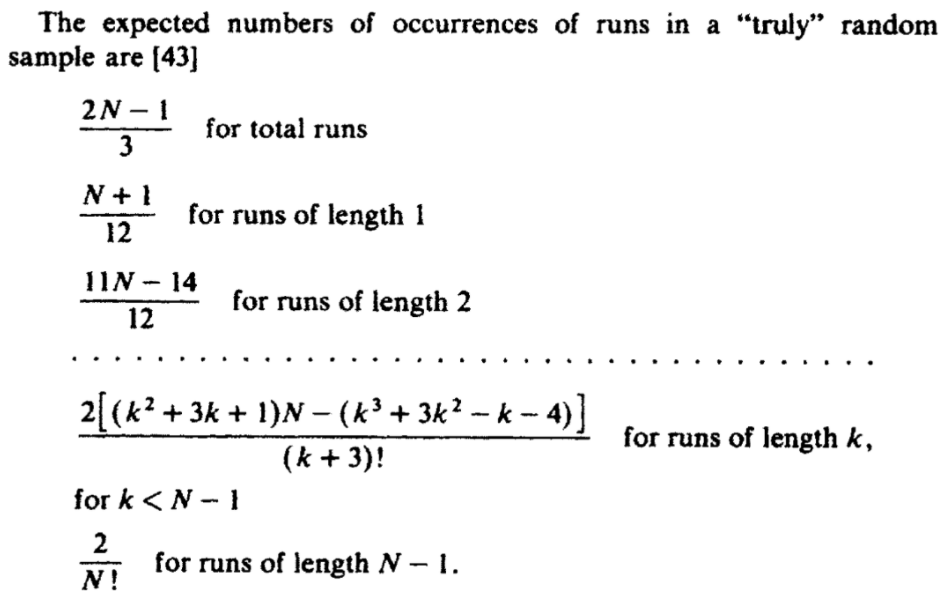
\includegraphics{./1.png}
\caption{Illustration of the model structure.}
\end{figure}

\hypertarget{regressors}{%
\subsubsection{10-2. Regressors}\label{regressors}}

Electricity consumption is highly correlated to the number of household
members of the respondent. When there are not too many household
members, with more members, the quantity of consumption decreases,
probably due to the fact that people tend to share the kitchen. However,
the effect diminishes gradually when there are many household members
(around 5-8).

\begin{center}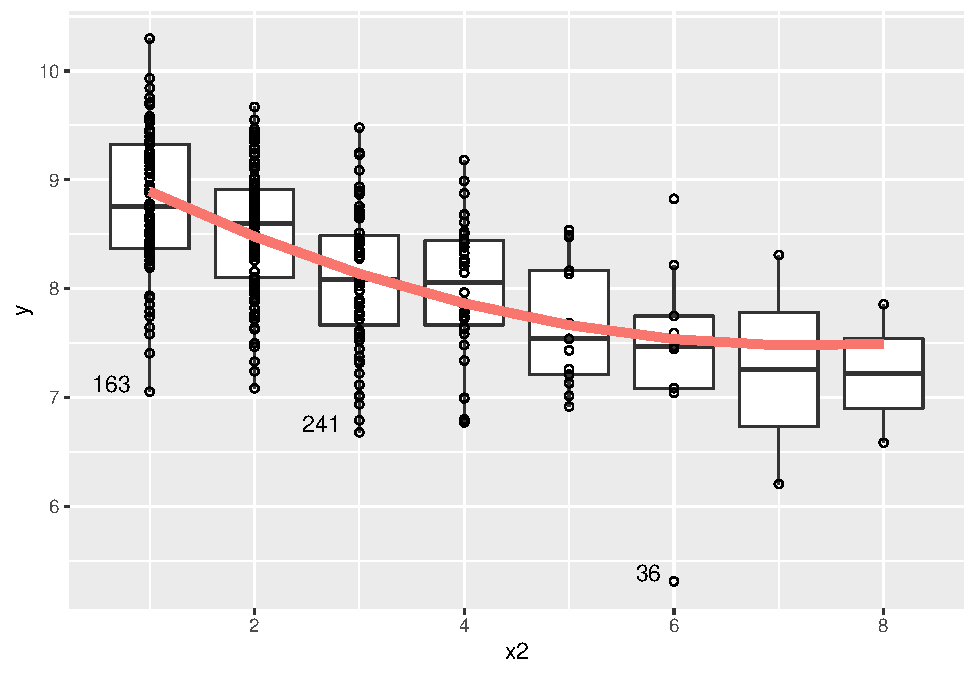
\includegraphics{main_files/figure-latex/unnamed-chunk-47-1} \end{center}

Because \texttt{y} is the log of average electricity consumptions, the
final relationship between electricity consumptions and numbers of
household members and numbers of rooms are:

As for the effect of number of rooms on electricity consumptions,

\begin{center}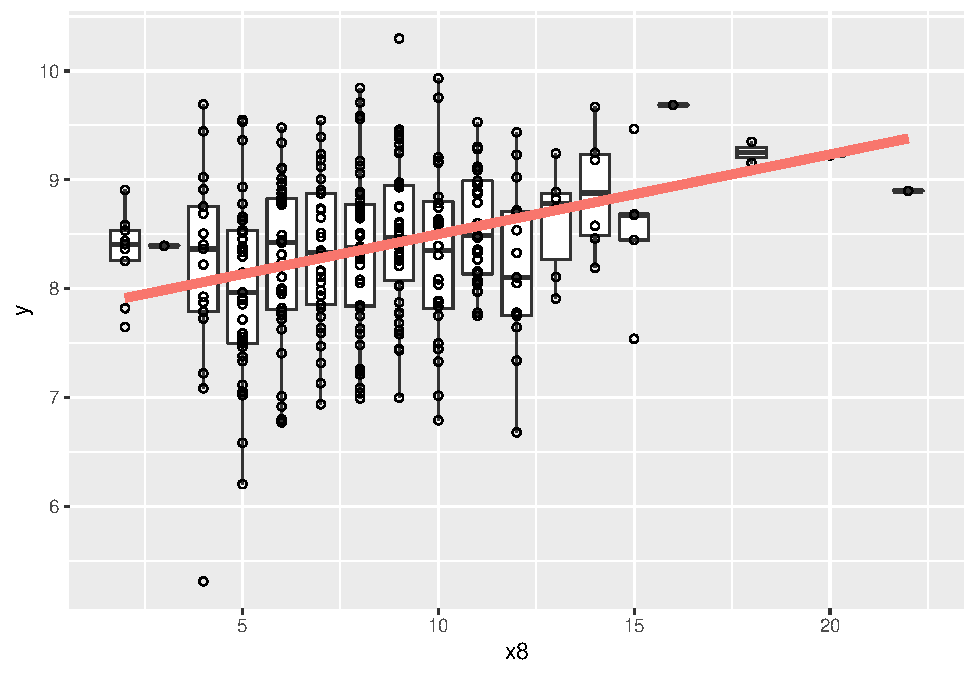
\includegraphics{main_files/figure-latex/unnamed-chunk-48-1} \end{center}

\hypertarget{orthogonalization-of-multiple-regressors}{%
\subsubsection{10-3. Orthogonalization of Multiple
Regressors}\label{orthogonalization-of-multiple-regressors}}

\begin{Shaded}
\begin{Highlighting}[]
\NormalTok{mods[[}\DecValTok{8}\NormalTok{]] <-}
\StringTok{  }\NormalTok{dat_}\DecValTok{2} \OperatorTok
\StringTok{  }\KeywordTok{mutate}\NormalTok{(}\DataTypeTok{z1 =} \KeywordTok{lm}\NormalTok{(x2 }\OperatorTok{~}\StringTok{ }\DecValTok{1}\NormalTok{)}\OperatorTok{$}\NormalTok{residuals) }\OperatorTok
\StringTok{  }\KeywordTok{mutate}\NormalTok{(}\DataTypeTok{z2 =} \KeywordTok{lm}\NormalTok{(x8 }\OperatorTok{~}\StringTok{ }\NormalTok{x2 }\OperatorTok{+}\StringTok{ }\DecValTok{1}\NormalTok{)}\OperatorTok{$}\NormalTok{residuals) }\OperatorTok
\StringTok{  }\KeywordTok{mutate}\NormalTok{(}\DataTypeTok{x2.2 =}\NormalTok{ x2}\OperatorTok{^}\DecValTok{2}\NormalTok{) }\OperatorTok
\StringTok{  }\KeywordTok{mutate}\NormalTok{(}\DataTypeTok{z3 =} \KeywordTok{lm}\NormalTok{(x2}\FloatTok{.2} \OperatorTok{~}\StringTok{ }\NormalTok{x2 }\OperatorTok{+}\StringTok{ }\NormalTok{x8 }\OperatorTok{+}\StringTok{ }\DecValTok{1}\NormalTok{)}\OperatorTok{$}\NormalTok{residuals) }\OperatorTok
\StringTok{  }\NormalTok{\{}\KeywordTok{lm}\NormalTok{(y }\OperatorTok{~}\StringTok{ }\NormalTok{z1 }\OperatorTok{+}\StringTok{ }\NormalTok{z2 }\OperatorTok{+}\StringTok{ }\NormalTok{z3, }\DataTypeTok{data =}\NormalTok{ .)\}}
\end{Highlighting}
\end{Shaded}

\begin{verbatim}
#> lm(formula = y ~ z1 + z2 + z3, data = .)
\end{verbatim}

\begin{table}[H]
\centering
\begin{tabular}{lllll}
\toprule
term & estimate & std.error & statistic & p.value\\
\midrule
(Intercept) & 8.370 & 0.033 & 249.9 & 0.0e+00\\
z1 & -0.257 & 0.024 & -10.5 & 3.4e-22\\
z2 & 0.066 & 0.011 & 6.1 & 4.1e-09\\
z3 & 0.036 & 0.012 & 2.9 & 4.1e-03\\
\bottomrule
\end{tabular}
\end{table}

\begin{table}[H]
\centering
\begin{tabular}{lllllllllll}
\toprule
r.squared & adj.r.squared & sigma & statistic & p.value & df & logLik & AIC & BIC & deviance & df.residual\\
\midrule
0.35 & 0.34 & 0.58 & 52 & 5.6e-27 & 4 & -259 & 528 & 546 & 99 & 295\\
\bottomrule
\end{tabular}
\end{table}

The intercept in \texttt{mods{[}{[}8{]}{]}} (8.37009) can be interpreted
as the exptected value for an individual with average values of
\texttt{x2}, \texttt{x8} and \texttt{I(x2\^{}2)}, which can be verified
by the prediction using \texttt{mods{[}{[}7{]}{]}}.

\begin{Shaded}
\begin{Highlighting}[]
\NormalTok{( }\FloatTok{8.77946} \OperatorTok{-}\StringTok{ }\FloatTok{0.52071} \OperatorTok{*}\StringTok{ }\KeywordTok{mean}\NormalTok{(dat_}\DecValTok{2}\OperatorTok{$}\NormalTok{x2) }\OperatorTok{+}\StringTok{ }\FloatTok{0.07329} \OperatorTok{*}\StringTok{ }\KeywordTok{mean}\NormalTok{(dat_}\DecValTok{2}\OperatorTok{$}\NormalTok{x8) }\OperatorTok{+}\StringTok{ }
\StringTok{  }\FloatTok{0.03563} \OperatorTok{*}\StringTok{ }\KeywordTok{mean}\NormalTok{(dat_}\DecValTok{2}\OperatorTok{$}\NormalTok{x2}\OperatorTok{^}\DecValTok{2}\NormalTok{) ) }\OperatorTok{-}\StringTok{ }\FloatTok{8.37009} \OperatorTok{<=}\StringTok{ }\FloatTok{1e-4}
\end{Highlighting}
\end{Shaded}

\begin{verbatim}
#> [1] TRUE
\end{verbatim}

Since the standard errors in \texttt{mods{[}{[}8{]}{]}} are smaller than
those in \texttt{mods{[}{[}7{]}{]}}, \texttt{mods{[}{[}8{]}{]}} is used
to conduct inference. Particularly, \texttt{se} for \texttt{Intercept}
is reduced by 75.48\%, and \texttt{se}s for first two regressors are
reduced by 71.75\% and 2.41\%. The estimations for the last term are
exactly the same, which is expected.

\begin{verbatim}
#>                   2.5 %      97.5 %
#> (Intercept)  8.30417224  8.43600027
#> z1          -0.30490653 -0.20881311
#> z2           0.04473184  0.08775875
#> z3           0.01138835  0.05986556
\end{verbatim}

To reduce average electricity consumptions, people are encouraged to
live together in houses with fewer rooms.

\hypertarget{one-sided-t-test-of-mods1}{%
\subsection{\texorpdfstring{11. One-Sided t-Test of
\texttt{mods{[}{[}1{]}{]}}}{11. One-Sided t-Test of mods{[}{[}1{]}{]}}}\label{one-sided-t-test-of-mods1}}

\begin{Shaded}
\begin{Highlighting}[]
\NormalTok{mods[[}\DecValTok{1}\NormalTok{]] }\OperatorTok
\StringTok{  }\KeywordTok{summary}\NormalTok{() }\OperatorTok
\StringTok{  }\NormalTok{\{}\KeywordTok{pt}\NormalTok{(}\KeywordTok{coef}\NormalTok{(.)[}\DecValTok{2}\NormalTok{, }\DecValTok{3}\NormalTok{], mods[[}\DecValTok{1}\NormalTok{]]}\OperatorTok{$}\NormalTok{df, }\DataTypeTok{lower =} \OtherTok{FALSE}\NormalTok{)\} }\OperatorTok
\StringTok{  }\NormalTok{\{. }\OperatorTok{<=}\StringTok{ }\KeywordTok{qchisq}\NormalTok{(}\FloatTok{0.95}\NormalTok{, }\DecValTok{1}\NormalTok{, }\DataTypeTok{lower.tail =} \OtherTok{TRUE}\NormalTok{, }\DataTypeTok{log.p =} \OtherTok{FALSE}\NormalTok{)\}}
\end{Highlighting}
\end{Shaded}

\begin{verbatim}
#> [1] TRUE
\end{verbatim}

\end{document}
